% Options for packages loaded elsewhere
\PassOptionsToPackage{unicode}{hyperref}
\PassOptionsToPackage{hyphens}{url}
%
\documentclass[
]{article}
\usepackage{amsmath,amssymb}
\usepackage{iftex}
\ifPDFTeX
  \usepackage[T1]{fontenc}
  \usepackage[utf8]{inputenc}
  \usepackage{textcomp} % provide euro and other symbols
\else % if luatex or xetex
  \usepackage{unicode-math} % this also loads fontspec
  \defaultfontfeatures{Scale=MatchLowercase}
  \defaultfontfeatures[\rmfamily]{Ligatures=TeX,Scale=1}
\fi
\usepackage{lmodern}
\ifPDFTeX\else
  % xetex/luatex font selection
\fi
% Use upquote if available, for straight quotes in verbatim environments
\IfFileExists{upquote.sty}{\usepackage{upquote}}{}
\IfFileExists{microtype.sty}{% use microtype if available
  \usepackage[]{microtype}
  \UseMicrotypeSet[protrusion]{basicmath} % disable protrusion for tt fonts
}{}
\makeatletter
\@ifundefined{KOMAClassName}{% if non-KOMA class
  \IfFileExists{parskip.sty}{%
    \usepackage{parskip}
  }{% else
    \setlength{\parindent}{0pt}
    \setlength{\parskip}{6pt plus 2pt minus 1pt}}
}{% if KOMA class
  \KOMAoptions{parskip=half}}
\makeatother
\usepackage{xcolor}
\usepackage[margin=1in]{geometry}
\usepackage{longtable,booktabs,array}
\usepackage{calc} % for calculating minipage widths
% Correct order of tables after \paragraph or \subparagraph
\usepackage{etoolbox}
\makeatletter
\patchcmd\longtable{\par}{\if@noskipsec\mbox{}\fi\par}{}{}
\makeatother
% Allow footnotes in longtable head/foot
\IfFileExists{footnotehyper.sty}{\usepackage{footnotehyper}}{\usepackage{footnote}}
\makesavenoteenv{longtable}
\usepackage{graphicx}
\makeatletter
\def\maxwidth{\ifdim\Gin@nat@width>\linewidth\linewidth\else\Gin@nat@width\fi}
\def\maxheight{\ifdim\Gin@nat@height>\textheight\textheight\else\Gin@nat@height\fi}
\makeatother
% Scale images if necessary, so that they will not overflow the page
% margins by default, and it is still possible to overwrite the defaults
% using explicit options in \includegraphics[width, height, ...]{}
\setkeys{Gin}{width=\maxwidth,height=\maxheight,keepaspectratio}
% Set default figure placement to htbp
\makeatletter
\def\fps@figure{htbp}
\makeatother
\setlength{\emergencystretch}{3em} % prevent overfull lines
\providecommand{\tightlist}{%
  \setlength{\itemsep}{0pt}\setlength{\parskip}{0pt}}
\setcounter{secnumdepth}{-\maxdimen} % remove section numbering
\ifLuaTeX
  \usepackage{selnolig}  % disable illegal ligatures
\fi
\usepackage{bookmark}
\IfFileExists{xurl.sty}{\usepackage{xurl}}{} % add URL line breaks if available
\urlstyle{same}
\hypersetup{
  pdftitle={Predicting Temperature with Monthly Global Average Methane Concentrations},
  pdfauthor={Jingze Dai, Rachael Stephan, \& Zhuocheng Zhang},
  hidelinks,
  pdfcreator={LaTeX via pandoc}}

\title{Predicting Temperature with Monthly Global Average Methane
Concentrations}
\author{Jingze Dai, Rachael Stephan, \& Zhuocheng Zhang}
\date{April 25, 2025}

\begin{document}
\maketitle

\section{Introduction}\label{introduction}

Greenhouse gases (GHG) are natural, atmospheric gases that can absorb
infrared radiation\footnote{Mann, M.E. (2025, April 11). greenhouse gas.
  Encyclopedia Britannica.
  \url{https://www.britannica.com/science/greenhouse-gas}}. GHGs will
reabsorb heat energy emitted by Earth and retain it within the
atmosphere, re-radiating heat back towards the
surface\textsuperscript{1}. This phenomena is known as the greenhouse
effect. Therefore, GHGs are important determinants of Earth's energy
budget and resulting climate\textsuperscript{1}. Concentrations of
greenhouse gases will naturally oscillate and there are other external
climate drivers as well (e.g., Milankovich cycles)\textsuperscript{1}.
However, the anthropogenic consumption of fossil fuels since the
Industrial Revolution have resulted in elevated concentrations of
GHGs\textsuperscript{1}. The most influential greenhouse gases with
regards to contribution to the greenhouse effect are carbon dioxide,
methane, and water\textsuperscript{1}.

Methane is commonly regarded as the second most important GHG compared
to carbon dioxide - especially considering methane has lower atmospheric
concentrations, but carbon dioxide and methane are difficult to compare
due to their residence time and radiative forcing
capabilities\footnote{MIT Climate (2024, January 4). Why do we compare
  methane to carbon dioxide over a 100-year timeframe? Are we
  underrating the importance of methane emissions? MIT Climate Portal.
  tps://climate.mit.edu/ask-mit/why-do-we-compare-methane-carbon-dioxide-over-100-year-timeframe-are-we-underrating}.
Methane has a more potent radiative forcing (i.e., higher heat
retention) but a residence time on the order of decades compared to
carbon dioxide's centuries\textsuperscript{1}. Assuming an equal amount
of each gas is released, this will result in methane having more power
over climate warming than carbon dioxide at small time
scales\textsuperscript{2}. Over 20 years in this scenario, methane will
be 80 times as powerful as carbon dioxide\textsuperscript{2}. Over the
next 100 years in this scenario, methane will be 28 times as powerful as
carbon dioxide\textsuperscript{2}. Therefore, methane is an important
consideration for near-future climate considerations, such as within our
lifetime.

Two of the major contributors to methane emissions are agricultural
practices and fossil fuels\footnote{Raymond, P., \& Hamburg, S. (2024,
  November 18). Yale experts explain methane emissions. Yale
  Sustainability.
  \url{https://sustainability.yale.edu/explainers/yale-experts-explain-methane-emissions}}.
The fermentation during the digestion process in cattle is the primary
source of agricultural methane. It is estimated that up to 264 pounds of
methane worldwide are emitted from cattle annually\footnote{U.S.
  Environmental Protection Agency. (2020, October). Agriculture and
  aquaculture: Food for thought.
  \url{https://www.epa.gov/snep/agriculture-and-aquaculture-food-thought}}.
Methane emitted through fossil fuels are caused by extraction leaks,
crude oil processing, and transportation of the fossil fuels. This
results in an estimated global annual emission of 120 million metric
tons\footnote{International Energy Agency. (2024). Global Methane
  Tracker 2024: Key findings. IEA.
  \url{https://www.iea.org/reports/global-methane-tracker-2024/key-findings}}.

Monitoring atmospheric GHG concentrations is important for climate
monitoring and tracking the effectiveness of climate change mitigation
-- including in the green energy transition. This report will
investigate the temporal trends in methane concentrations considering
the exogenous factors of beef production and socioeconomic factors (as a
proxy for fossil fuel consumption). We will use our methane projections
to extrapolate trends in climate, represented by temperature anomalies
based on an averaged climate from 1901 to 2000.

\section{Data Sources}\label{data-sources}

The following data sources were used in this analysis and their
respective wrangling is described below.

\begin{enumerate}
\def\labelenumi{\arabic{enumi}.}
\tightlist
\item
  \emph{Globally averaged methane concentration data}
\end{enumerate}

\begin{itemize}
\tightlist
\item
  Frequency: monthly
\item
  Units: ppb
\item
  Format: csv file
\item
  Source:
  \href{https://gml.noaa.gov/ccgg/trends_ch4/}{\textcolor{blue}{NOAA Global Monitoring Laboratory}}
\end{itemize}

The initial methane data set was an excel \texttt{.csv} file with
columns of the year, month, decimal year, average methane concentration,
average uncertainty, trend value, and trend uncertainty on a single
sheet. It was processed as follows:

\begin{itemize}
\tightlist
\item
  The header and data were read in as separate data frames because of
  the excel file formatting.
\item
  The header information was set as the column names for the data.
\item
  A date was created using the month and year columns using lubridate's
  \texttt{make\_date} function. The day was assumed to be the first of
  the month.
\item
  Data set was verified for missing data - none were present.
\item
  Data frames were saved as the full data, training period data, and
  test period data. The training and testing periods are expanded upon
  in the methods section.
\end{itemize}

\begin{enumerate}
\def\labelenumi{\arabic{enumi}.}
\setcounter{enumi}{1}
\tightlist
\item
  \emph{Globally averaged temperature anomaly data (based on a 1901-2000
  average)}
\end{enumerate}

\begin{itemize}
\tightlist
\item
  Frequency: monthly
\item
  Units: degrees Celsius
\item
  Format: csv file
\item
  Source:
  \href{https://www.ncei.noaa.gov/access/monitoring/climate-at-a-glance/global/time-series}{\textcolor{blue}{NOAA National Center for Environmental Information}}
\end{itemize}

The initial temperature anomaly data set was an excel \texttt{.csv} file
with columns of the date and temperature anomaly on a single sheet. It
was processed as follows:

\begin{itemize}
\tightlist
\item
  Only the data was read into a data frame from the excel file.
\item
  The column names for the data frame were manually set.
\item
  The date column was converting into date format using lubridate's
  \texttt{ym} function.
\item
  Data set was verified for missing data - none were present.
\item
  Data frames were saved as the full data, training period data, and
  test period data. The training and testing periods are expanded upon
  in the methods section.
\end{itemize}

\begin{enumerate}
\def\labelenumi{\arabic{enumi}.}
\setcounter{enumi}{2}
\tightlist
\item
  \emph{Aggregated global beef production}
\end{enumerate}

\begin{itemize}
\tightlist
\item
  Frequency: yearly
\item
  Units: metric tons
\item
  Format: csv file
\item
  Source:
  \href{https://www.fas.usda.gov/data/production/commodity/0111000}{\textcolor{blue}{U.S. Department of Agriculture}}
\end{itemize}

\begin{enumerate}
\def\labelenumi{\arabic{enumi}.}
\setcounter{enumi}{3}
\tightlist
\item
  \emph{Socioeconomic factors data set including consumer price index
  (CPI), industrial production, merchandise exports, and merchandise
  imports.}
\end{enumerate}

\begin{itemize}
\tightlist
\item
  Frequency: monthly
\item
  Units: index (2005=100)
\item
  Format: csv file
\item
  Source
  \href{https://www.dallasfed.org/research/econdata#international}{\textcolor{blue}{Federal Reserve Bank of Dallas}}
\end{itemize}

It was processed as follows: - The date column was converting into date
format using lubridate's \texttt{ymd} function. - Use the
\texttt{filter} function to select the dates that match the methane
data, and then save to the processed \texttt{.csv} file. - There is no
missing data, and there is also no outliers.

\subsection{Data Summary}\label{data-summary}

The data frames were not combined for analysis, but the relevant factors
have been merged into a data frame for summary purposes below (Table 1).
All of the monthly data is shown in a single data frame (Table 2) and
yearly data (i.e., beef production) is shown in another data frame
(Table 3).

\begin{longtable}[]{@{}
  >{\raggedright\arraybackslash}p{(\columnwidth - 16\tabcolsep) * \real{0.2157}}
  >{\raggedright\arraybackslash}p{(\columnwidth - 16\tabcolsep) * \real{0.2157}}
  >{\raggedright\arraybackslash}p{(\columnwidth - 16\tabcolsep) * \real{0.0588}}
  >{\raggedright\arraybackslash}p{(\columnwidth - 16\tabcolsep) * \real{0.0784}}
  >{\raggedright\arraybackslash}p{(\columnwidth - 16\tabcolsep) * \real{0.0588}}
  >{\raggedright\arraybackslash}p{(\columnwidth - 16\tabcolsep) * \real{0.0980}}
  >{\raggedright\arraybackslash}p{(\columnwidth - 16\tabcolsep) * \real{0.0882}}
  >{\raggedright\arraybackslash}p{(\columnwidth - 16\tabcolsep) * \real{0.0980}}
  >{\raggedright\arraybackslash}p{(\columnwidth - 16\tabcolsep) * \real{0.0882}}@{}}
\caption{Summary statistics for all of the variables used in the
analysis from July 1, 1983 to November 1, 2024, Beef Production is
provided until 2023.}\tabularnewline
\toprule\noalign{}
\begin{minipage}[b]{\linewidth}\raggedright
Variable
\end{minipage} & \begin{minipage}[b]{\linewidth}\raggedright
Units
\end{minipage} & \begin{minipage}[b]{\linewidth}\raggedright
Count
\end{minipage} & \begin{minipage}[b]{\linewidth}\raggedright
Mean
\end{minipage} & \begin{minipage}[b]{\linewidth}\raggedright
SD
\end{minipage} & \begin{minipage}[b]{\linewidth}\raggedright
Min
\end{minipage} & \begin{minipage}[b]{\linewidth}\raggedright
Max
\end{minipage} & \begin{minipage}[b]{\linewidth}\raggedright
Pct25
\end{minipage} & \begin{minipage}[b]{\linewidth}\raggedright
Pct75
\end{minipage} \\
\midrule\noalign{}
\endfirsthead
\toprule\noalign{}
\begin{minipage}[b]{\linewidth}\raggedright
Variable
\end{minipage} & \begin{minipage}[b]{\linewidth}\raggedright
Units
\end{minipage} & \begin{minipage}[b]{\linewidth}\raggedright
Count
\end{minipage} & \begin{minipage}[b]{\linewidth}\raggedright
Mean
\end{minipage} & \begin{minipage}[b]{\linewidth}\raggedright
SD
\end{minipage} & \begin{minipage}[b]{\linewidth}\raggedright
Min
\end{minipage} & \begin{minipage}[b]{\linewidth}\raggedright
Max
\end{minipage} & \begin{minipage}[b]{\linewidth}\raggedright
Pct25
\end{minipage} & \begin{minipage}[b]{\linewidth}\raggedright
Pct75
\end{minipage} \\
\midrule\noalign{}
\endhead
\bottomrule\noalign{}
\endlastfoot
Methane & ppb & 497 & 1781.27 & 70.59 & 1625.96 & 1941.81 & 1739.23 &
1820.87 \\
Temperature.Anomaly & degrees Celsius & 497 & 0.61 & 0.29 & 0.02 & 1.44
& 0.39 & 0.8 \\
CPI & index (2005=100) & 497 & 93.25 & 57.34 & 4.35 & 208.43 & 45.95 &
139.02 \\
Exports & index (2005=100) & 497 & 105.18 & 71.27 & 14.42 & 259.8 & 38.7
& 173.05 \\
Imports & index (2005=100) & 497 & 82.87 & 31.05 & 30.64 & 140.91 & 47.9
& 112.91 \\
Industrial.Production & index (2005=100) & 497 & 99.84 & 38.8 & 43.65 &
177.6 & 62.6 & 132.51 \\
Beef Production & metric tons (million) & 41 & 619.72 & 81.01 &
490.34412 & 765.6081 & 545.37624 & 692.5579 \\
\end{longtable}

\begin{longtable}[]{@{}
  >{\raggedright\arraybackslash}p{(\columnwidth - 12\tabcolsep) * \real{0.1341}}
  >{\raggedleft\arraybackslash}p{(\columnwidth - 12\tabcolsep) * \real{0.0976}}
  >{\raggedleft\arraybackslash}p{(\columnwidth - 12\tabcolsep) * \real{0.2439}}
  >{\raggedleft\arraybackslash}p{(\columnwidth - 12\tabcolsep) * \real{0.0610}}
  >{\raggedleft\arraybackslash}p{(\columnwidth - 12\tabcolsep) * \real{0.0976}}
  >{\raggedleft\arraybackslash}p{(\columnwidth - 12\tabcolsep) * \real{0.0976}}
  >{\raggedleft\arraybackslash}p{(\columnwidth - 12\tabcolsep) * \real{0.2683}}@{}}
\caption{First 10 cases of global methane (ppb), temperature anomaly
(degrees celsius), and socioeconomic indicators}\tabularnewline
\toprule\noalign{}
\begin{minipage}[b]{\linewidth}\raggedright
Date
\end{minipage} & \begin{minipage}[b]{\linewidth}\raggedleft
Methane
\end{minipage} & \begin{minipage}[b]{\linewidth}\raggedleft
Temperature.Anomaly
\end{minipage} & \begin{minipage}[b]{\linewidth}\raggedleft
CPI
\end{minipage} & \begin{minipage}[b]{\linewidth}\raggedleft
Exports
\end{minipage} & \begin{minipage}[b]{\linewidth}\raggedleft
Imports
\end{minipage} & \begin{minipage}[b]{\linewidth}\raggedleft
Industrial.Production
\end{minipage} \\
\midrule\noalign{}
\endfirsthead
\toprule\noalign{}
\begin{minipage}[b]{\linewidth}\raggedright
Date
\end{minipage} & \begin{minipage}[b]{\linewidth}\raggedleft
Methane
\end{minipage} & \begin{minipage}[b]{\linewidth}\raggedleft
Temperature.Anomaly
\end{minipage} & \begin{minipage}[b]{\linewidth}\raggedleft
CPI
\end{minipage} & \begin{minipage}[b]{\linewidth}\raggedleft
Exports
\end{minipage} & \begin{minipage}[b]{\linewidth}\raggedleft
Imports
\end{minipage} & \begin{minipage}[b]{\linewidth}\raggedleft
Industrial.Production
\end{minipage} \\
\midrule\noalign{}
\endhead
\bottomrule\noalign{}
\endlastfoot
1983-07-01 & 1625.96 & 0.23 & 4.35 & 14.42 & 30.64 & 43.65 \\
1983-08-01 & 1628.05 & 0.36 & 4.41 & 14.72 & 31.78 & 44.29 \\
1983-09-01 & 1638.43 & 0.42 & 4.47 & 15.05 & 31.32 & 44.77 \\
1983-10-01 & 1644.80 & 0.22 & 4.53 & 15.00 & 33.81 & 44.78 \\
1983-11-01 & 1642.61 & 0.35 & 4.59 & 15.23 & 32.02 & 45.15 \\
1983-12-01 & 1639.54 & 0.24 & 4.65 & 15.28 & 31.74 & 45.61 \\
1984-01-01 & 1638.73 & 0.31 & 4.71 & 15.80 & 35.95 & 45.97 \\
1984-02-01 & 1638.82 & 0.20 & 4.77 & 16.00 & 36.07 & 46.24 \\
1984-03-01 & 1640.87 & 0.31 & 4.84 & 16.03 & 36.68 & 46.20 \\
1984-04-01 & 1643.96 & 0.12 & 4.90 & 15.66 & 38.07 & 46.17 \\
\end{longtable}

\begin{longtable}[]{@{}rr@{}}
\caption{First 10 cases of beef production (metric tons)}\tabularnewline
\toprule\noalign{}
Year & Beef.Production \\
\midrule\noalign{}
\endfirsthead
\toprule\noalign{}
Year & Beef.Production \\
\midrule\noalign{}
\endhead
\bottomrule\noalign{}
\endlastfoot
1983 & 490.3441 \\
1984 & 504.3934 \\
1985 & 513.5100 \\
1986 & 531.0788 \\
1987 & 530.7524 \\
1988 & 535.6858 \\
1989 & 537.9553 \\
1990 & 553.5117 \\
1991 & 553.5116 \\
1992 & 545.3762 \\
\end{longtable}

All of the identified variables have a relatively strong correlation
with each other (Fig. 1). The highest correlation between exogenous
variables and methane is CPI with 0.97. The correlation between
temperature and methane is 0.87.

\begin{figure}
\centering
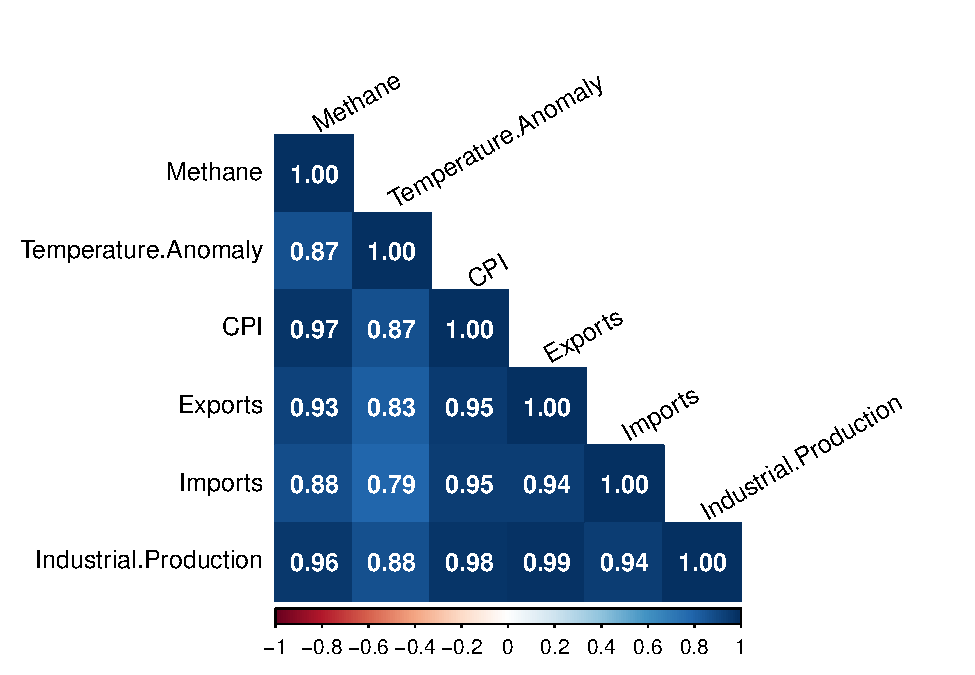
\includegraphics{Final_Report_files/figure-latex/unnamed-chunk-4-1.pdf}
\caption{Correlation Between All Monthly Variables}
\end{figure}

\section{Analysis}\label{analysis}

\subsection{Libraries}\label{libraries}

The following libraries were used in the analysis:

\begin{itemize}
\tightlist
\item
  \texttt{tidyverse}: a collection of R packages with similar grammar
  data structures used to tidy and process data, including
  \texttt{ggplot2} and \texttt{lubridate} which are for graphing and
  handling dates respectively.
\item
  \texttt{forecast}: methods and tools used to produce and analyze
  univariate time series forecasts
\item
  \texttt{cowplot}: an addition to \texttt{ggplot2} used to align
  figures
\item
  \texttt{Kendall}: contains the Kendall and Mann-Kendall statistical
  methods
\item
  \texttt{tseries}: tools for time series analysis and computational
  finance
\item
  \texttt{corrplot}: a visual exploratory tool for plotting correlation
  matrices
\item
  \texttt{smooth}: tools for state space modelling
\end{itemize}

\subsection{Training and Test Periods}\label{training-and-test-periods}

The training period was designated as July 1, 1983 to December 1, 2021.
The test period was designated as January 1, 2022 to November 1, 2024.
These periods were used to filter the data to create test and training
data subsets.

\subsection{Methane Concentration
Predictions}\label{methane-concentration-predictions}

The methane data has an increasing trend with a seasonal component (Fig.
2).

\begin{figure}
\centering
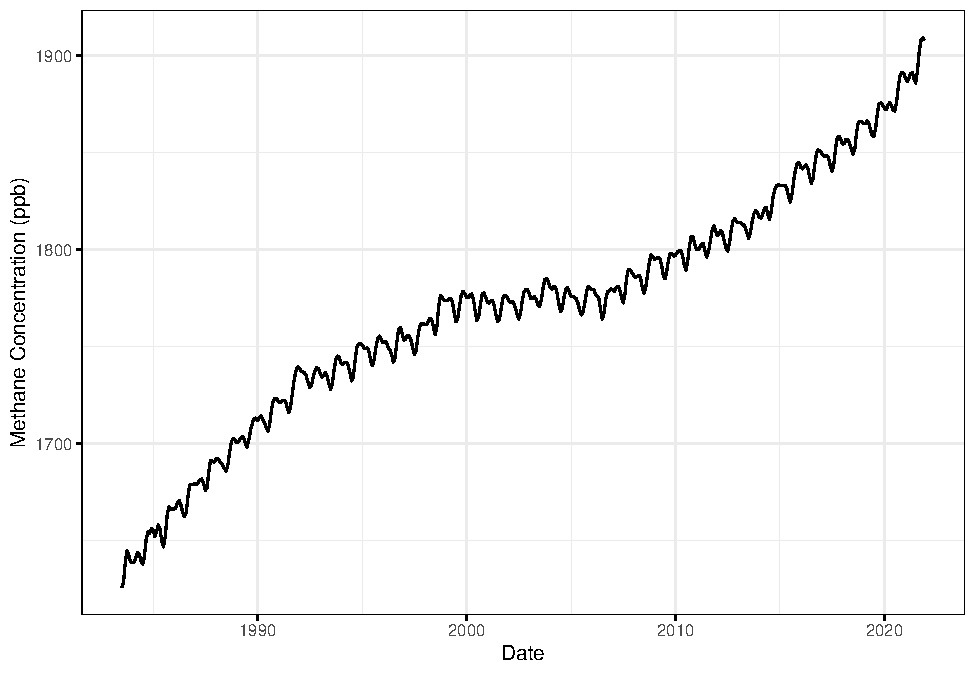
\includegraphics{Final_Report_files/figure-latex/unnamed-chunk-5-1.pdf}
\caption{Globally Averaged Methane Concentrations From July 1, 1983 -
November 1, 2024}
\end{figure}

Decomposing the methane time series confirms a positive trend with a
seasonal component (Fig. 3). The random component is relatively evenly
distributed, but there may be some seasonality or other periodic
component remaining because the peaks and troughs appear to be fairly
regular.

\begin{figure}
\centering
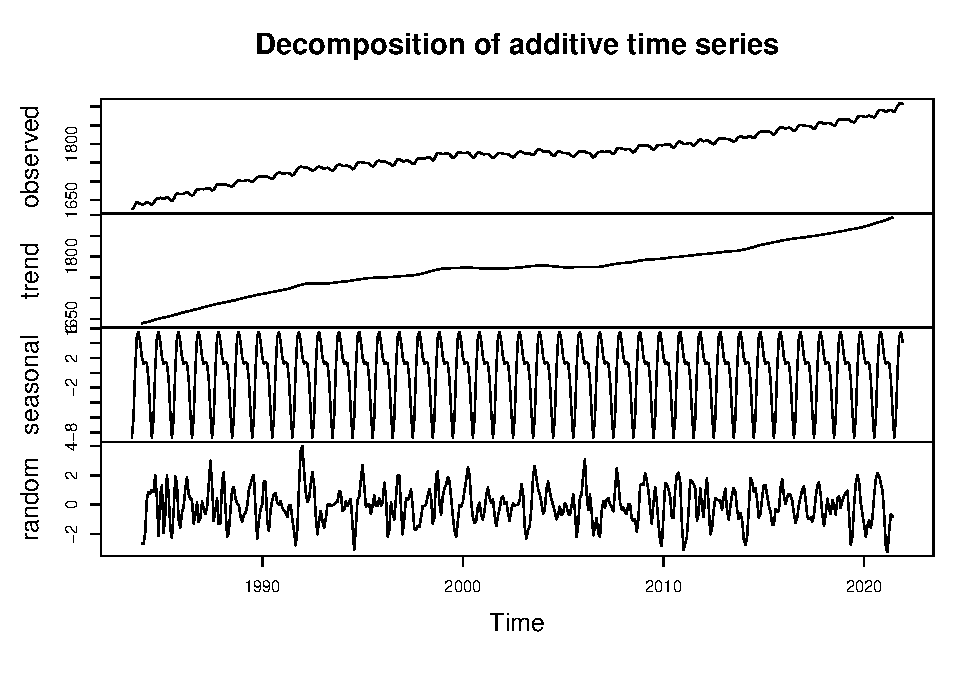
\includegraphics{Final_Report_files/figure-latex/unnamed-chunk-6-1.pdf}
\caption{The components of the methane time series}
\end{figure}

The ACF plot shows a gradual decay and the PACF plot shows a sharp drop
off after lag 1 (Fig. 4). This indicates temperature may have an
auto-regressive component to the methane time series. The seasonality is
not strongly visible in the ACF plot.

\begin{figure}
\centering
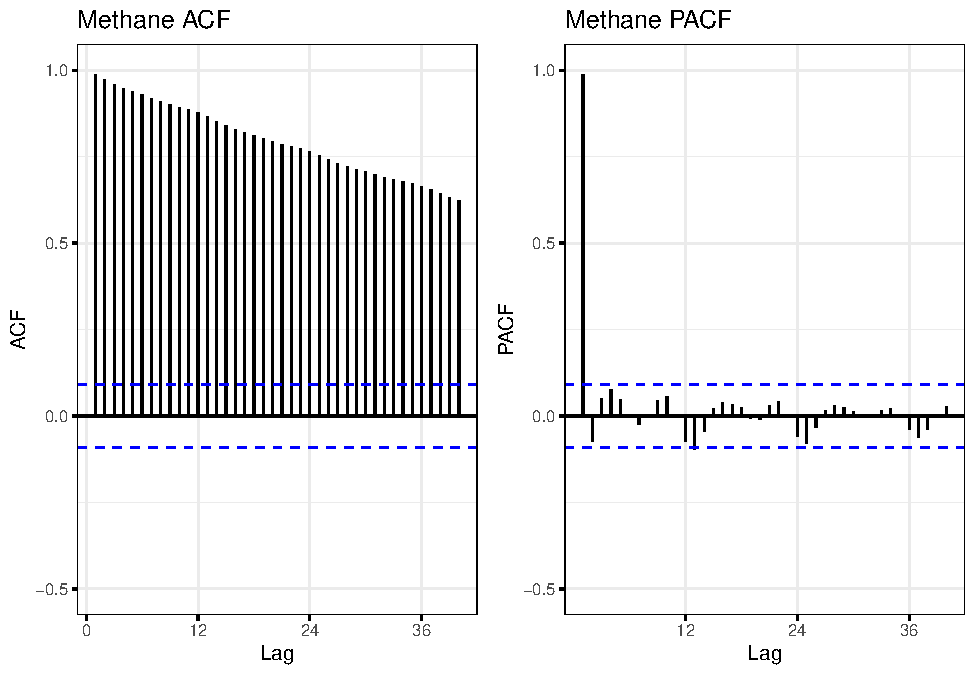
\includegraphics{Final_Report_files/figure-latex/unnamed-chunk-7-1.pdf}
\caption{The autocorrelation and partial autocorrelation plots of the
methane time series}
\end{figure}

Before fitting into an ARIMA model, we preformed Augmented Dickey-Fuller
(ADF) test and Mann-Kendall test to check for deterministic and
stochastic trends in the methane dataset.

\begin{verbatim}
## [1] "Mann-Kendall Test"
\end{verbatim}

\begin{verbatim}
## Score =  102531 , Var(Score) = 10992237
## denominator =  106491
## tau = 0.963, 2-sided pvalue =< 2.22e-16
\end{verbatim}

From the results of the Mann-Kendall test, the p-value is less than
0.05, indicating a significant trend. The test score of 102531 indicates
a strong increasing deterministic trend, which agrees with the upward
trend in the decomposed series.

\begin{verbatim}
## 
##  Augmented Dickey-Fuller Test
## 
## data:  deseasoned
## Dickey-Fuller = -1.7274, Lag order = 7, p-value = 0.6932
## alternative hypothesis: stationary
\end{verbatim}

From the ADF test, the p-value of 0.6932 is greater than the
significance level of 0.05, meaning that there is not enough evidence to
reject the null hypothesis. This series appears to have stochastic trend
that changes over time.

Next, the following models were used to predict methane concentrations
without the use of exogenous variables.

\begin{enumerate}
\def\labelenumi{\arabic{enumi}.}
\tightlist
\item
  ARIMA using \texttt{auto.arima} and adding the decomposed seasonality
  (from \texttt{decompose}) afterwards
\item
  SARIMA using \texttt{auto.arima} with Fourier terms
\item
  ARIMA with Fourier terms with \texttt{auto.arima} function
\item
  ETS Model with the \texttt{stlf} function
\item
  Neural Network Model with the \texttt{nnetar} function
\item
  TBATS Model with the \texttt{tbats} function
\item
  State Space Model - Exponential Smoothing with the \texttt{es}
  function
\item
  State Space Model - BSM with the \texttt{StructTS} function
\end{enumerate}

The following models were used to predict methane concentrations with
the use of exogenous variables (i.e., using the \texttt{xreg} term).

As presented in the variable correlation matrix plot, socioeconomic
factors exhibit strong colinearity. To deal with this issue, we propose
two forms of method:

\begin{enumerate}
\def\labelenumi{\alph{enumi})}
\tightlist
\item
  Use a non-linear model (e.g., Neural Network) to incorporate multiple
  variables simultaneously.
\item
  Include only one variable at a time in the linear model.
\end{enumerate}

The models with the best predictor is as follows:

\begin{enumerate}
\def\labelenumi{\arabic{enumi}.}
\tightlist
\item
  Arima using \texttt{auto.arima} function, using industrial production
  variable
\item
  Arima with Fourier terms with \texttt{auto.arima} function, using
  industrial production variable
\item
  SARIMA using `auto.arima with industrial production variable
\item
  TBATS using \texttt{tbats} function, with cpi variable
\item
  Neural Network Model with the \texttt{nnetar} function, with cpi and
  export variables
\item
  STL+Arima Model with cpi variable
\item
  State Space Model with industrial production variable
\end{enumerate}

Given the vast number of possible variable combinations, we created a
variable portfolio and the model combination, both involving and not
involving exogenous variables. we explored all possible combinations of
variables and models by creating a loop function to iterate through all
combinations and perform forecasting. The total, we evaluated over
60,000 combinations. The performance of all of the models were examined
with the \texttt{accuracy} function and the methane test data subset. We
therefore choose the variable which has lower \texttt{MAPE} score from
these loops. All of these forecasts closely follow the trend in methane
(Fig. 5).

\begin{longtable}[]{@{}
  >{\raggedleft\arraybackslash}p{(\columnwidth - 4\tabcolsep) * \real{0.0625}}
  >{\raggedright\arraybackslash}p{(\columnwidth - 4\tabcolsep) * \real{0.8125}}
  >{\raggedleft\arraybackslash}p{(\columnwidth - 4\tabcolsep) * \real{0.1250}}@{}}
\caption{The top five methane concentration models and their performance
statistics sorted by MAPE.}\tabularnewline
\toprule\noalign{}
\begin{minipage}[b]{\linewidth}\raggedleft
Rank
\end{minipage} & \begin{minipage}[b]{\linewidth}\raggedright
Model
\end{minipage} & \begin{minipage}[b]{\linewidth}\raggedleft
MAPE
\end{minipage} \\
\midrule\noalign{}
\endfirsthead
\toprule\noalign{}
\begin{minipage}[b]{\linewidth}\raggedleft
Rank
\end{minipage} & \begin{minipage}[b]{\linewidth}\raggedright
Model
\end{minipage} & \begin{minipage}[b]{\linewidth}\raggedleft
MAPE
\end{minipage} \\
\midrule\noalign{}
\endhead
\bottomrule\noalign{}
\endlastfoot
1 & ets\_nn\_nnExoSE\_nnFourier\_sses\_ssesExoSE & 0.0540012 \\
2 & arimaFourier\_nn\_nnExoSE\_nnFourier\_sses\_ssesExoSE\_stlArimaExoSE
& 0.0549470 \\
3 &
arimaFourier\_ets\_nn\_nnExoSE\_nnFourier\_sarimaExoSE\_sses\_ssesExoSE
& 0.0551739 \\
4 & ets\_nn\_nnExoSE\_nnFourier\_sses\_ssesExoSE\_stlArimaExoSE &
0.0551828 \\
5 & arimaFourier\_nn\_nnExoSE\_nnFourier\_sses\_ssesExoSE & 0.0552185 \\
\end{longtable}

\begin{figure}
\centering
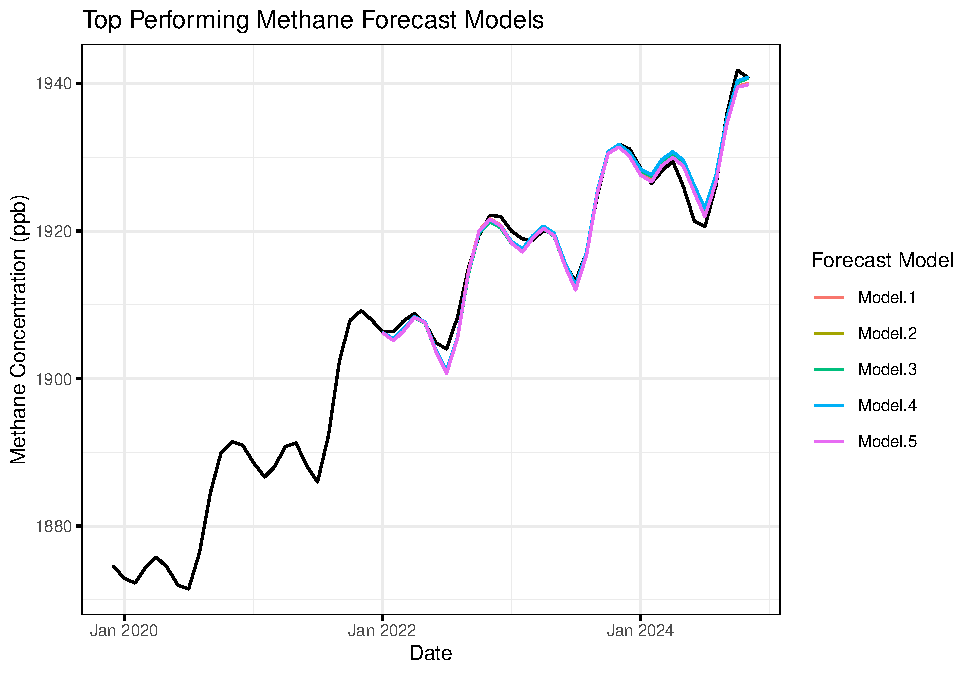
\includegraphics{Final_Report_files/figure-latex/unnamed-chunk-11-1.pdf}
\caption{The top five performing methane concentration forecast models.
Models are numbered by their performance by MAPE and the full title can
be found in Table 4}
\end{figure}

\textbf{TALK ABOUT TOP 3 MODELS AND LOOK AT THEIR RESIDUALS}

\newpage

\subsection{Temperature Anomaly
Predictions}\label{temperature-anomaly-predictions}

Temperature anomaly data was examined using the \texttt{decompose}
function (Fig. 6 and 7). The temperature anomaly data has a general
increasing trend. There is a annual seasonal trend but it is smaller
than the random errors and not easily visible. However, it does have a
similar shape to the methane seasonality. The remainders do not appear
to have any trends and there are few outliers.

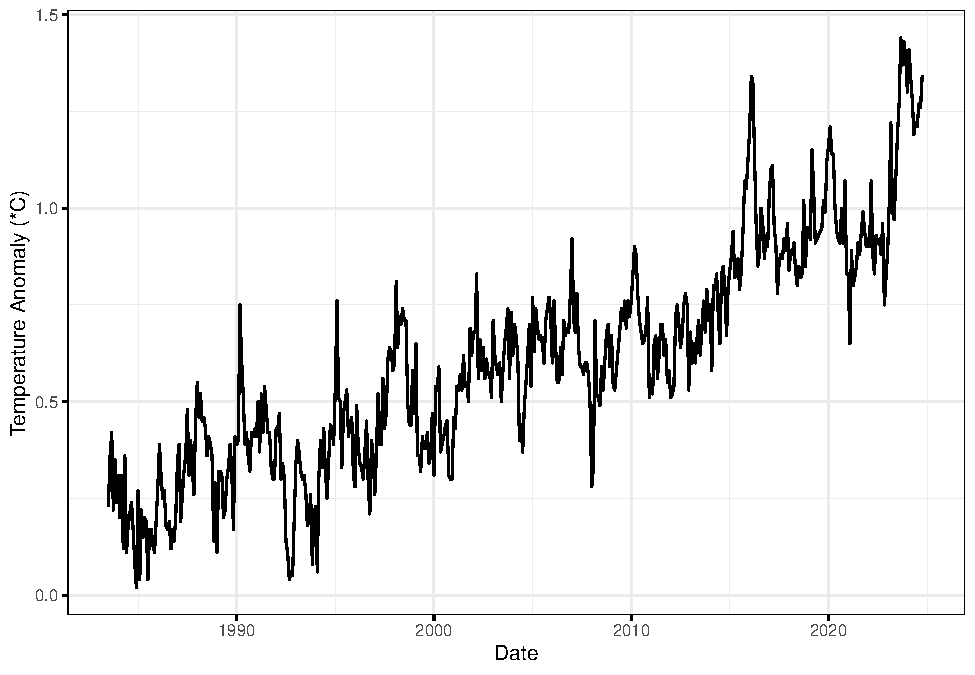
\includegraphics{Final_Report_files/figure-latex/unnamed-chunk-12-1.pdf}
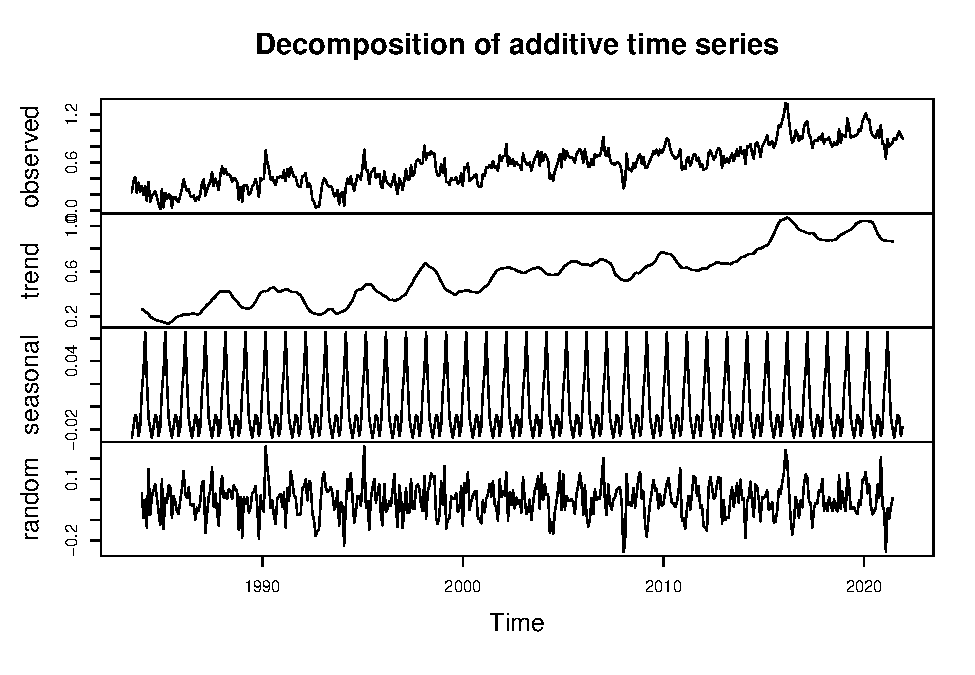
\includegraphics{Final_Report_files/figure-latex/unnamed-chunk-13-1.pdf}

The ACF plot shows a gradual decay and the PACF plot shows a sharp drop
off after lag 2 (Fig. 8). This indicates temperature may have an
auto-regressive component to the model. There does appear to be a slight
seasonal scalloping in the ACF plot.

\begin{figure}
\centering
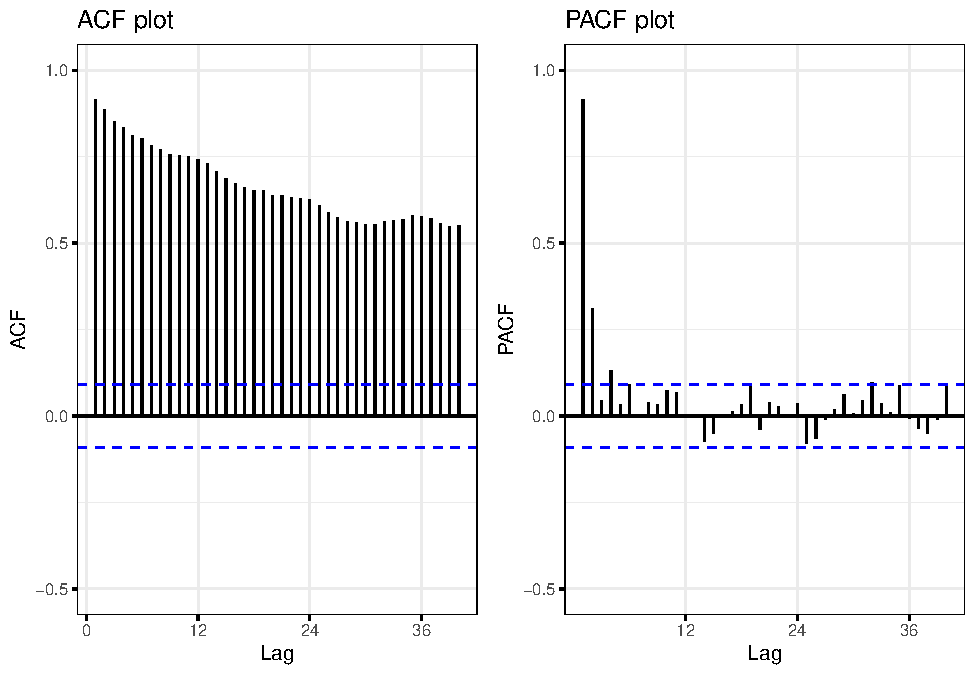
\includegraphics{Final_Report_files/figure-latex/unnamed-chunk-14-1.pdf}
\caption{The autocorrelation and partial autocorrelation plots of the
temperature time series}
\end{figure}

The following models were used to predict methane concentrations without
the use of exogenous variables.

\begin{enumerate}
\def\labelenumi{\arabic{enumi}.}
\tightlist
\item
  SARIMA
\item
  ARIMA with Fourier
\end{enumerate}

The following models were used to predict methane concentrations with
the use of exogenous variables (i.e., using the \texttt{xreg} term).

\begin{enumerate}
\def\labelenumi{\arabic{enumi}.}
\tightlist
\item
  ARIMAX with Fourier
\item
  SARIMAX
\item
  Neural Network
\item
  Random Forest
\end{enumerate}

All of the above models were averaged together in every possible
combination. The performance of all of the models were examined with the
\texttt{accuracy} function and the methane test data subset. The best
performing model was the SARIMAX model. However, the MAPE was much
higher than in our methane forecasts (Table 5), and the forecast does
not accurately reflect the most recent upwards trends in temperature
(Fig. 9). The temperature trended upwards for most of the data record,
but recently that trend stabilized. Therefore, the models are likely
biased towards recent events and did not capture the shift back to an
upwards trend.

\begin{longtable}[]{@{}
  >{\raggedleft\arraybackslash}p{(\columnwidth - 12\tabcolsep) * \real{0.0658}}
  >{\raggedright\arraybackslash}p{(\columnwidth - 12\tabcolsep) * \real{0.2895}}
  >{\raggedleft\arraybackslash}p{(\columnwidth - 12\tabcolsep) * \real{0.1316}}
  >{\raggedleft\arraybackslash}p{(\columnwidth - 12\tabcolsep) * \real{0.1316}}
  >{\raggedleft\arraybackslash}p{(\columnwidth - 12\tabcolsep) * \real{0.1316}}
  >{\raggedleft\arraybackslash}p{(\columnwidth - 12\tabcolsep) * \real{0.1316}}
  >{\raggedleft\arraybackslash}p{(\columnwidth - 12\tabcolsep) * \real{0.1184}}@{}}
\caption{The top five temperature anomaly models and their performance
statistics sorted by MAPE.}\tabularnewline
\toprule\noalign{}
\begin{minipage}[b]{\linewidth}\raggedleft
Rank
\end{minipage} & \begin{minipage}[b]{\linewidth}\raggedright
Model
\end{minipage} & \begin{minipage}[b]{\linewidth}\raggedleft
ME
\end{minipage} & \begin{minipage}[b]{\linewidth}\raggedleft
RSME
\end{minipage} & \begin{minipage}[b]{\linewidth}\raggedleft
MAE
\end{minipage} & \begin{minipage}[b]{\linewidth}\raggedleft
MPE
\end{minipage} & \begin{minipage}[b]{\linewidth}\raggedleft
MAPE
\end{minipage} \\
\midrule\noalign{}
\endfirsthead
\toprule\noalign{}
\begin{minipage}[b]{\linewidth}\raggedleft
Rank
\end{minipage} & \begin{minipage}[b]{\linewidth}\raggedright
Model
\end{minipage} & \begin{minipage}[b]{\linewidth}\raggedleft
ME
\end{minipage} & \begin{minipage}[b]{\linewidth}\raggedleft
RSME
\end{minipage} & \begin{minipage}[b]{\linewidth}\raggedleft
MAE
\end{minipage} & \begin{minipage}[b]{\linewidth}\raggedleft
MPE
\end{minipage} & \begin{minipage}[b]{\linewidth}\raggedleft
MAPE
\end{minipage} \\
\midrule\noalign{}
\endhead
\bottomrule\noalign{}
\endlastfoot
1 & sarimax & 0.0978695 & 0.2032856 & 0.1721584 & 5.932950 & 14.71139 \\
2 & rfExo\_sarimax & 0.1354008 & 0.2351881 & 0.1938629 & 9.141813 &
16.11481 \\
3 & arimaFourier\_sarimax & 0.1375237 & 0.2411710 & 0.1956617 & 9.298260
& 16.14617 \\
4 & arimaxFourier\_sarimax & 0.1375237 & 0.2411710 & 0.1956617 &
9.298260 & 16.14617 \\
5 & sarima\_sarimax & 0.1510658 & 0.2437155 & 0.1979484 & 10.607708 &
16.27890 \\
\end{longtable}

\begin{figure}
\centering
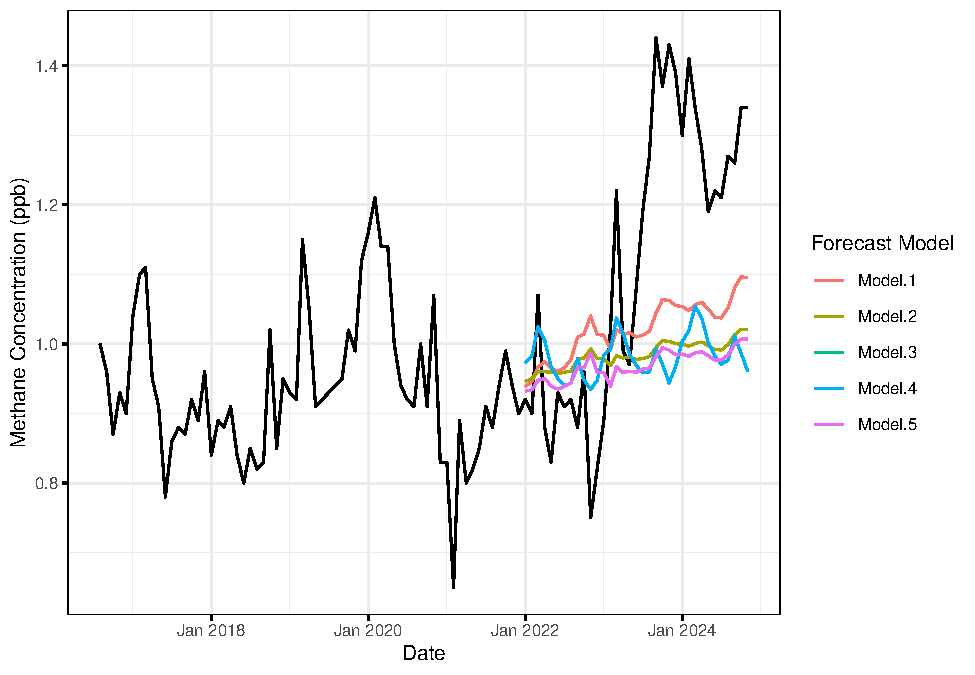
\includegraphics{Final_Report_files/figure-latex/unnamed-chunk-16-1.pdf}
\caption{The top five performing methane concentration forecast models.
Models are numbered by their performance by MAPE and the full title can
be found in Table 5}
\end{figure}

\begin{figure}

{\centering 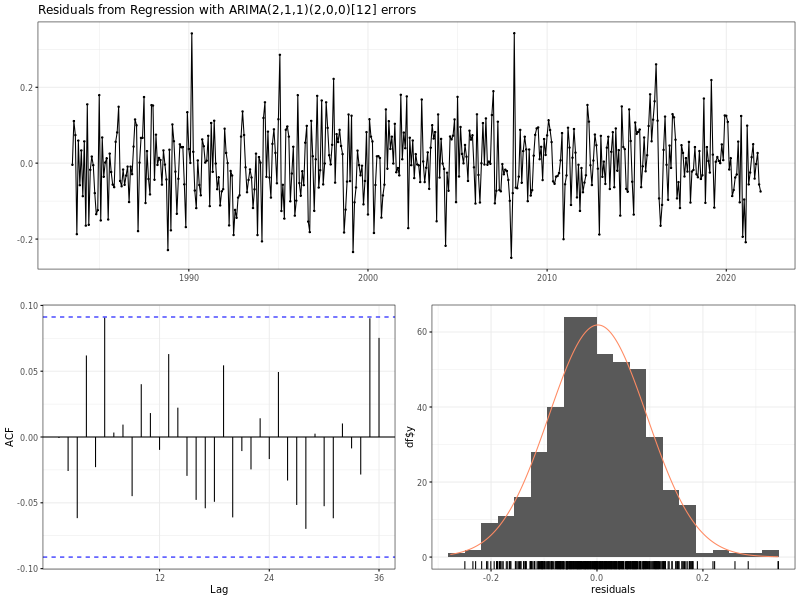
\includegraphics[width=0.8\linewidth]{./Forecasts/residuals_sarimax} 

}

\caption{Residual analysis of the Temperature anomaly SARIMAX forecast}\label{fig:unnamed-chunk-17}
\end{figure}

We used the SARIMAX model to predict temperature for 3 years into the
future, using the whole data set as a training data set and assuming
that the current climate scenario does not drastically change (Fig. 10).
The future project appears to be strongly dominated by the seasonality
of methane concentrations with a bias for the stable trend over the past
couple of years. It does not seem likely that this forecast will
accurately reflect the future temperatures.

\begin{figure}
\centering
\includegraphics{Final_Report_files/figure-latex/unnamed-chunk-18-1.pdf}
\caption{Future temperature forecasts based on the sarimax model with
exogenous variable of methane.}
\end{figure}

\section{Conclusions}\label{conclusions}

Using a variety of statistical models, both involving and not involving
exogenous variables of socioeconomic factors, methane concentrations
were able to be accurately forecasted. The most successful model (MAPE =
0.0540012) was a average of the following models:

\begin{itemize}
\tightlist
\item
  STL + ETS
\item
  Neural Network
\item
  Neural Network with Exogenous variable of socioeconomic factor
\item
  Neural Network with Fourier terms
\item
  Steady State model with exponential smoothing
\item
  Steady State model with exponential smoothing with Exogenous variable
  of socioeconomic factor
\item
  STL + ARIMA model with exogenous variable of socioeconomic factors
\end{itemize}

We hypothesize that the best performing model was an average of many
models because the models had different strengths in capturing the trend
and seasonality. The behavior of the methane concentrations was also
very regular, which made it easy to accurately predict the
concentrations. The socioeconomic factors, which were a proxy for
release from fossil fuels, resulted in some of the highest performing
time series. All of the socioeconomic factors had a high correlation
with methane, which likely helped to improve predictions. From our
predictions, we can conclude that methane concentrations have a clear
seasonality and are consistently increasing. We do not think these
models could be improved much with the current dataset.

Temperature forecasts were best predicted using a SARIMAX model with the
exogenous variable of methane concentrations. The SARIMAX model did not
perform well in the training data. The behavior was driven by the
methane exogenous variable, as seen in the familiar seasonal trends that
are not previously prevalent in the temperature anomaly data. It also
seems that the model is also biased by the recent stabilization in the
temperature anomaly trend. More models would have to be run to try and
circumvent this issue. We could also be attempting to forecast at an
inopportune timepoint (i.e., at the start of a change in the trend).
Correspondingly, our forecasts of temperature into the future are likely
inaccurate as well. More models would have to be run to try and
circumvent this issue. Perhaps models with either a longer memory or a
quicker response to changes in trends will perform better. Another
potential avenue for exploration is other exogenous variables, such as
other GHGs. Temperature is likely regulated by a number of different
factors and methane alone does not fully capture the relationships.

\end{document}
